\chapter{Anwendungsfall und Prototyp}
\label{chapter:prototype}

In den Kapiteln zuvor wurde in das Thema durch Grundlagen und eine Vorstellung der einzelnen Streaming Frameworks eingeführt. Dieses Kapitel beschreibt eine Methode zur Messung der Performance. Es wird zunächst das Messverfahren gezeigt, die Messumgebung und die Anforderungen an die Prototypen beschrieben. Um einem Vergleich zwischen den Streaming Frameworks auf Entwicklungsebene näher zu kommen, ist es notwendig eine allgemeine Anwendung in einer homogenen Umgebung zu entwickeln und bereitzustellen. Dazu werden zuerst die funktionalen Anforderungen und anschließend die nichtfunktionalen Anforderungen in schriftlicher und darstellerischer Form beschrieben.

\section{Funktionale Anforderung}
\label{sec:funktAnforderung}
Die funktionalen Anforderungen tragen dazu bei die Anwendung zu implementieren. In den folgenden Listen werden Kriterien für die Prototypen der einzelnen Streaming Frameworks definiert. Das Use-Case-Diagramm zeigt die Muss-Kriterien für den Anwender in Abbildung \ref{fig:useCaseMussKriterien}

\textbf{Muss-Kriterien:}
\begin{description}
  \item[M3] Paketierung der Implementierungen mit Apache Maven	
	\item[M2] Ausführung der Implementierungen unter Java und dem Betriebssystem Linux
	\item[M1] Ausführung einer Implementierung auf einem Single-Node-Cluster	
	\item[M4] Ausführung einer Implementierung von konstanten Größe von 100 Byte-Daten (statischer Payload)
	\item[M5] Ausführung einer Implementierung von variablen Größe von Daten (dynamischer Payload)
	\item[M6] Aufnahme von Daten: aktueller Nachrichten pro Sekunde und CPU-Belastung während der Ausführung einer Implementierung in  separaten Dateien 
	\item[M7] Während der Ausführung, anzeige der Daten pro Streaming Framework auf einer Webseite - Übersichtsseite
\end{description}

\textbf{Soll-Kriterien:}
\begin{description}
  \item[S1] Ausführung einer Implementierung auf verschiedenen Rechnersystemen (Professional Workstation, Notebook, Virtuelle Maschine)
	\item[S2] die Dynamische Implementierungen sollen Wörter aus einem offen und frei zugänglichen großen Datensatzes zählen und die Anzahl der höchsten 5 Wörter, sowie das Wort selbst pro Sekunde automatisch anzeigen
	\item[S3] Die Inhalte auf der Webseite sollen über Javascript-Trigger aktualisiert werden
\end{description}

\textbf{Kann-Kriterien:}
\begin{description}
  \item[K1] Ausführung der Implementierungen auf Multi-Node-Cluster
	\item[K2] Ausführung auf proprietären Betriebssystemen
\end{description}

\textbf{Abgrenzungskriterien:}
\begin{description}
  \item[A1] Für die prototypische Entwicklung werden erst in einem weiterführenden Konzept Unit- und Verhaltens-Tests eingesetzt
	\item[A2] Die Darstellung von Information auf einer Webseite benötigt beim Prototypen keine Serverseitige Absicherung
\end{description}


\begin{figure}[htb!]
\centering
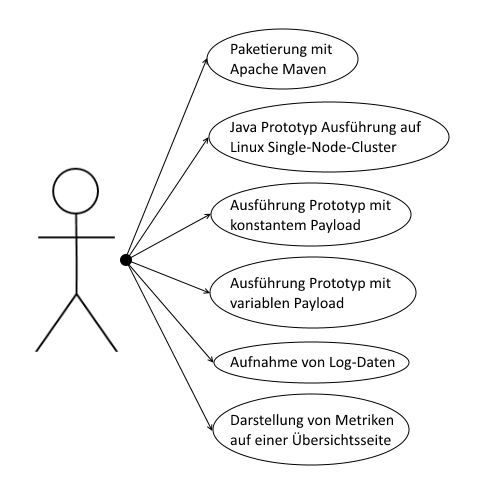
\includegraphics[width=0.65\textwidth]{bilder/useCaseMussKriterien.png}
\caption{Muss-Kriterien Use-Case-Diagramm
\label{fig:useCaseMussKriterien}}
\end{figure}

Nachdem die Kriterien vorgestellt wurden wird als nächste der Einsatzbereich und die Umgebung gezeigt.

\section{Nichtfunktionale Kriterien}
\label{sec:einsatzUmgebung}

Die Implementierungen der Prototypen werden hauptsächlich in einem wissenschaftlichen Studium eingesetzt. Als Zielgruppe können Wissenschaftler in der Informationstechnologie, Datenanalysten und Entwickler aus dem Bereich der Datenverarbeitung von zeitkritischen Daten und der Daten einer großen Menge, ein Interesse finden. Betrieben werden die Prototypen auf einem Notebook, in einer virtuellen Instanz und auf einer professionellen Workstation. Alle Rechnereinheiten werden über ein Switch verkabelt. Dabei wird ein homogenes Netz gebildet. 

Um Störgrößen zu vermeiden ist eine Verbindung in das Internet und das Intranet nicht vorgesehen und eine feste Verdrahtung essentiell. Kabellose Verbindungen werden aufgrund größerer Störempfindlichkeit wie zum Beispiel Kanalauslöschung nicht unterstützt. Das System wird mit kostenloser Open-Source Software entwickelt, dabei wird auf eine gute Wartbarkeit und Performance geachtet.

Angeschlossene Fremdrechner benötigen für die Darstellung der Übersichtsseite einen aktuellen Webbrowser\footnote{Webbrowser: \url{https://www.mozilla.org/de/firefox/desktop/}}. Die Nachrichten werden innerhalb der Streaming Frameworks binär und nach außen, zur Übersichtsseite als \gls{glo:json} übertragen. Für die Eingabedaten wird ein freies, offenes und großes Shakespear-Datensatz \citeint{dataset:shakespeare:1994:CWW} benutzt. Im folgenden Kapitel werden die Implementierungen der Prototypen dokumentiert.




\section{Prototypdokumentation}
\label{sec:prototypeDocumentation}